\documentclass[sigconf]{acmart}

\AtBeginDocument{%
  \providecommand\BibTeX{{%
    \normalfont B\kern-0.5em{\scshape i\kern-0.25em b}\kern-0.8em\TeX}}}

\usepackage{dblfloatfix}
\usepackage{mathtools}
\usepackage{hyperref}
\usepackage[htt]{hyphenat}

\begin{document}

\title{Comparative Study of Conversational Search Engine Retrieval Pipelines}
\subtitle{Group ID: \#5}

% AUTHORS:
\author{Til Mohr}
\affiliation{}
\email{tv.mohr@stud.uis.no}

\author{Ishaac Ourahou}
\affiliation{}
\email{i.ourahou@stud.uis.no}

% DATE:
\date{\today}



\begin{abstract}
In our master's degree program, we delved into the realms of information retrieval and text mining. Our group project focuses on developing a system capable of searching for specific passages within a conversation. This entails considering the historical context of previous exchanges when interpreting the current user's query. The system reformulates the user's query to better align with the conversation's overarching topic and then seeks the most relevant passages from a vast collection of 8.8 million documents, specifically from the MS MARCO document collection. We initially create a baseline information retrieval pipeline, which serves as our foundational reference. We then explore advanced techniques and methods in the field of conversational search engines. Our report concludes with a comparative analysis between the baseline system and our advanced retrieval mechanisms, outlining the strengths and shortcomings of our approaches, and offering conclusions.
\end{abstract}

\keywords{information retrieval, conversational search engine, conversational search system}

%% Remove copyright footer
\settopmatter{printacmref=false}
\setcopyright{none}
\renewcommand\footnotetextcopyrightpermission[1]{}
\pagestyle{plain}
%% ------------------------

%%
%% This command processes the author and affiliation and title
%% information and builds the first part of the formatted document.
\maketitle


\section{Introduction}\label{sec:intro}
With the rise of conversational agents like Amazon Alexa and Apple Siri, the ability to accurately and relevantly respond to user requests has become increasingly important. These agents are designed to interact fluidly with users, and the essence of their functionality rests on providing precise information in their responses.

Our project centers on building a conversational search engine, a system that not only addresses the user's immediate question but also takes into account previous queries and the ongoing conversation's topic. This provides a more holistic approach to the user's information needs. Initially, we will construct a basic architecture, establishing our baseline system. This baseline will serve as a comparison point against more sophisticated techniques. It's required, however, that even this foundational system meets or exceeds the performance of the reference system set by our project guides.

Our research will utilize the MS MARCO dataset, a comprehensive collection of 8.8 million documents. Efficiently retrieving relevant documents from this vast pool necessitates an indexing process, which we will execute using the \texttt{pyterrier} API.

Section \ref{sec:problem} will articulate the specific problem we aim to address. In Section \ref{sec:related} we will explore literature relevant to our retrieval pipelines. We will then elaborate on the methodologies behind our retrieval pipelines in Sections \ref{sec:baseline}, \ref{sec:baseline+rm3}, \ref{sec:doc2query-method}, and \ref{sec:doc2query-method+rm3}. Our report will conclude in Section \ref{sec:results}, where we evaluate and compare the effectiveness of our systems, highlighting the strengths and potential areas of enhancement in our advanced approaches.

The codebase for our project can be found on GitHub\footnote{URL: \url{https://github.com/CodingTil/2023_24---IRTM---Group-Project}}.

\section{Problem Statement}\label{sec:problem}
This project focuses on developing a Conversational Search Engine (CSE). What distinguishes a CSE from a traditional search engine is its inherent context-aware nature. In a CSE, queries asked by a user within a session are semantically interconnected. Rather than treating each query in isolation, a CSE leverages information from both the previous queries and the system's responses to those queries to retrieve relevant passages. It must cater to the continuous thread of a dialogue, while also being agile enough to accommodate sudden shifts in conversation topics. For every user query, the goal is to generate a ranked listing of the top 1000 passages out of an expansive 8.8 million document collection.

A vital component that sets a CSE apart is its query rewriting mechanism. This feature reformulates the presented query to better reflect the ongoing conversation topic. Figure \ref{figure:global_pipeline} offers a schematic representation of how the various stages of a CSE retrieval pipeline interact. Analogous to traditional search engines, a CSE also requires prior indexing of the document collection, enabling computationally efficient retrieval and ranking processes.

\begin{figure}[h]
	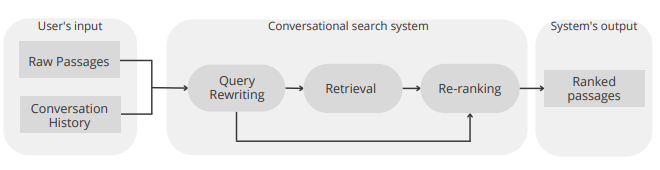
\includegraphics[width=7cm]{pipeline.png}
	\caption{Overall system's pipeline architecture}
	\label{figure:global_pipeline}
\end{figure}


\section{Related Work}\label{sec:related}
In this Section, we delve into pertinent research encompassing the realms of conversational search engines and the broader area of information retrieval. While certain highlighted studies do not directly cater to conversational search engines or explicit information retrieval, their techniques remain invaluable in various stages of the conversational retrieval process.

\subsection*{Pseudo-Relevance Feedback by Query Expansion}\label{sec:prf}
Oftentimes, queries entered by users are too short and include too little hint for the search engine to retrieve all relevant documents \cite{vaidyanathan2015query}. To counter this, the user-generated query must be reformulated to better reflect the user's informational needs. One approach to this is known as query expansion using relevance feedback: Assume we have a set of documents relevant to the user-generated query. One can then reformulate the query such that the retrieval system retrieves documents similar to the set of relevant documents, i.e. documents that are probably also relevant to the user's query. This expansion is accomplished by selecting keywords from the set of relevant documents and appending those to the query. Different strategies for this exist \cite{vaidyanathan2015query}.

However, in a real setting, we do not have a set of relevant documents. Instead, we can generate a set of documents that are hopefully relevant to the user's query, and then follow the same process. Since the relevance of the generated set of documents is unknown, this approach is called pseudo-relevance feedback. In order to retrieve this set, we can use the original user entered query to retrieve only the top $p$ documents. If $p$ is very small, it is likely that all those documents are relevant to the query. Expanding the query using those documents will then likely result in a better retrieval of all relevant documents \cite{vaidyanathan2015query}.

One particular technique for this is known as \texttt{RM3} \cite{abdul2004umass}. \texttt{RM3} uses relevance-based language models \cite{lavrenko2017relevance} to estimate the relevance of a word based on the word's probability in the language models of the (pseudo-)relevant documents. This relevance of the word to the query is then interpolated with the original query language model to avoid the query drifting too far away from the original query. The resulting language model is then used to generate a new query. Overall, the \texttt{RM3} approach can be parameterized in the number of documents to use for the pseudo-relevance feedback, the number of terms to add to the query, and the interpolation parameter \cite{abdul2004umass,lavrenko2017relevance,chen2022pseudo}.


\subsection*{Text-to-Text Transfer Transformer}\label{sec:t5}
The vast domain of natural language processing (NLP) revolves around the understanding of natural language, whether presented in text or speech form. NLP aspires to equip computers with the capability to grasp the depth of human language and harness this understanding to execute a range of tasks, such as text summarization, machine translation, and question answering. Given the diverse nature of these tasks in terms of their input, output, and underlying challenges, developing a unified model proficient across the entire spectrum poses a significant challenge.

Enter the Text-to-Text Transfer Transformer (\texttt{T5}) \cite{raffel2020exploring}. This work by Raffel et al. introduces transfer learning in NLP, aiming to craft a versatile model that can be used for any NLP problem. In essence, T5 models first learn the basics of language. Then, they're sharpened for particular tasks using targeted data. It's common to find models that have been trained in this manner for any specific NLP problem.

\subsection*{\texttt{doc2query} Document Expansion}\label{sec:doc2query}
Traditional retrieval techniques, such as \texttt{BM25}, rely primarily on term occurrences in both queries and documents. However, they often overlook the semantics of the content. As a result, documents that may be semantically relevant to a query might be scored as non-relevant due to differences in syntax or terminology. Dense retrieval methods, which emphasize semantic similarities between texts, can address this problem but are computationally taxing during retrieval.

A notable solution to this is the \texttt{doc\-2query} method proposed by Nogueira et al. \cite{nogueira2019document}. It employs a text-to-text transformer to convert documents into queries. By generating and appending a few of these transformed queries to the original document, classical retrieval methods show significantly improved performance. This is because these additional queries often capture semantic nuances similar to those in the actual query \cite{nogueira2019document,nogueira2019doc2query,pradeep2021expando}. Importantly, \texttt{doc\-2query} shifts the computational load to the indexing phase, ensuring minimal performance lag during retrieval. By leveraging the \texttt{T5} model, the authors further enhanced the query generation quality, leading to the variation known as \texttt{doc\-TTTTTquery}, \texttt{doc\--T5query}, or \texttt{doc\-2query\--T5} \cite{nogueira2019doc2query}.

\subsection*{\texttt{SPARTA} Sparse Retrieval}\label{sec:sparta}
\texttt{SPARTA}, introduced by Zhao et al. \cite{zhao2020sparta}, represents a nuanced take on sparse retrieval. At its core, it works by encoding documents into sparse representations during the indexing phase. These representations not only capture the document's actual content but also incorporate terms that are semantically resonant, even if they're not present in the document. This underlying principle echoes the rationale of approaches like \texttt{doc2query} and dense retrieval models.

Yet, where \texttt{SPARTA} differentiates itself is in its retrieval phase. Unlike dense retrieval models, it retrieves pertinent documents using straightforward index lookups, mirroring lexical retrieval strategies like \texttt{BM25} \cite{zhao2020sparta}.

However, in real-world applications, \texttt{SPARTA} faces challenges. Several other models, including \texttt{BM25} and \texttt{doc2query-T5}, surpass it in ranking efficacy. Additionally, its indexing footprint is substantially larger compared to alternatives like \texttt{doc2query-T5} \cite{thakur2021beir}.

\subsection*{\texttt{monoT5} \& \texttt{duoT5} Rerankers}\label{sec:rerankers}
\texttt{monoT5} and \texttt{duoT5} are neural re-rankers, also developed by Nogueira et al., which attempt to inject semantic understanding into the retrieval process \cite{nogueira2020document,nogueira2019multi}. Using the \texttt{T5} model, they re-rank a list of documents based on their semantic relevance to a given query. Specifically, \texttt{monoT5} processes a query and a single document, outputting a relevance score. In contrast, \texttt{duoT5} considers a query and two documents, determining which document is more relevant. Although \texttt{duoT5} offers a more nuanced ranking, its pairwise comparison method makes it computationally heavier. Hence, a staged re-ranking approach is proposed: first using \texttt{monoT5} for the top $k$ documents and subsequently applying \texttt{duoT5} to a smaller subset, the top $l$, where $l \ll k$ \cite{nogueira2019multi,pradeep2021expando}.


\subsection*{Expando-Mono-Duo Design Pattern}\label{sec:expando}
The same research team introduced a strategic pattern for integrating the above tools into retrieval pipelines, termed the Expando-Mono-Duo design pattern \cite{pradeep2021expando}. Here's how it works: During indexing, \texttt{doc2query-T5} is employed to enhance document representation and better the initial retrieval results from methods like \texttt{BM25}. The retrieved results are then re-ranked with \texttt{monoT5}. A selected top tier from this list undergoes another re-ranking using \texttt{duoT5}. Trials show that this composite approach leads to marked improvements in result quality across multiple evaluation metrics \cite{pradeep2021expando}.

\subsection*{Conversational Query Rewriting}\label{sec:cqr}

Conversational search engines distinguish themselves from standard search engines by determining document relevance through the entirety of a conversation, not just the immediate query. In conversational contexts, subsequent questions often lean on prior interactions, implying that previous questions and answers must be factored in when fetching relevant documents. However, there's also a need to cater to conversation shifts where the immediate query doesn't relate to preceding exchanges. Blindly considering the entire conversational history in such cases could detriment retrieval accuracy.

Elgohary et al. address this challenge with an innovative approach \cite{elgohary2019can}. They suggest reshaping the current query based on the overarching conversation. This reformulated query is designed to function autonomously within conventional retrieval pipelines. In essence, this technique extends the utility of standard search engines to conversational question-answering scenarios by introducing a preceding conversational query modification stage.

Employing text-to-text transformers, like \texttt{T5}, can be instrumental in achieving this rewrite. These models are nurtured to revamp the immediate query, factoring in the conversational backdrop. Studies validate the efficacy of this approach, highlighting its capacity to enhance the retrieval accuracy of traditional search engines in conversational contexts \cite{elgohary2019can,anantha2020open,Lajewska:2023:ECIR}.



\section{Baseline Method}\label{sec:baseline}
Our baseline method is inspired by the baseline method presented by Łajewska et al. \cite{Lajewska:2023:ECIR}. It is structured in the following sequence:
\begin{enumerate}
	\item	\texttt{T5} Query Rewriting
	\item	\texttt{BM25} Retrieval
	\item	Re-ranking
			\begin{enumerate}
				\item	Re-ranking using \texttt{monoT5}
				\item	Top-document re-ranking using \texttt{duoT5}
			\end{enumerate}
\end{enumerate}

\subsection{\texttt{T5} Query Rewriting}
In conversation search engines, query rewriting is the crucial component to include the semantics of the conversation history into the currently asked query, which results into a singular rewritten query that can be fed into the retrieval pipeline.

For this purpose, we include all the previously rewritten queries $q'_0 \dots q'_{n-1}$ of our conversation, as well as the response $r_{n-1}$ of the CSE to the previous rewritten query $q'_{n-1}$ into the current query $q_n$. This is done by concatenating the previous rewritten queries and the response into a single string:
\begin{align*}
	q'_n \coloneqq q'_0 \text{<sep>} \dots \text{<sep>} q'_{n-1} \text{<sep>} r_{n-1} \text{<sep>} q_n
\end{align*}
This approach resembles the approach taken by Łajewska et al. \cite{Lajewska:2023:ECIR}.

We have found through experimentation that this mere concatenation is insufficient to produce satisfiable results: The concatenated string is too long, and too much focus during the later retrieval is being put on $r_{n-1}$, which make responses sudden topic changes impossible.

Driven by these insights, we have turned our attention to other query rewriting techniques. \texttt{Pyterrier} provides the \texttt{Sequential\-Dependence} query rewriting method\footnote{URL: \url{https://pyterrier.readthedocs.io/en/latest/rewrite.html\#sequentialdependence}}. We have found, however, that this rewriter also does not produce the desired results.

Subsequent exploration led us to the \texttt{T5} neural query rewriter trained for conversational question rewriting, see Section \ref{sec:cqr}. With this method, $q'_n$ closely mirrored $q_n$, subtly infusing it with the conversation's context, particularly when no drastic topic alterations were identified. A valuable by-product was the concise nature of the rewritten query, a departure from the growing length observed previously. Since retrieval latency is a critical factor, we utilized a smaller \texttt{T5} model: \texttt{castorini\-/t5\--base\--canard}\footnote{URL: \url{https://huggingface.co/castorini/t5-base-canard}}

\subsection{\texttt{BM25} Retrieval}
We settled on the \texttt{BM25} retrieval method, a commonly used formula in the realm of information retrieval, for its simplicity and its deployment in the reference system, allowing for direct comparisons.

\subsection{Re-ranking}
The re-ranking stage of our baseline system consists of two stages: First, the top 1000 documents retrieved by the \texttt{BM25} retrieval method are re-ranked using the \texttt{monoT5} reranker. Afterwards, the top 50 documents of the previous re-ranking stage are rearranged using the \texttt{duoT5} reranker, see Section \ref{sec:rerankers}. The precise count of documents subject to reranking at each stage is a hyperparameter of our system, allowing to balance computational cost and result quality. These rerankers were implemented in the \texttt{pyterrier\_t5} library.\footnote{URL: \url{https://github.com/terrierteam/pyterrier_t5}} Again, since a low latency of our retrieval pipeline is crucial to us, we utilized smaller \texttt{T5} models: \texttt{castorini\-/monot5\--base\--msmarco}\footnote{URL: \url{https://huggingface.co/castorini/monot5-base-msmarco}} for \texttt{monoT5} and \texttt{castorini\-/duot5\--base\--msmarco}\footnote{URL: \url{https://huggingface.co/castorini/duot5-base-msmarco}} for \texttt{duoT5}.

\section{Incorporating Pseudo-Relevance Feedback into Our Baseline}\label{sec:baseline+rm3}

Recognizing the substantial performance enhancements associated with pseudo-relevance feedback, we felt compelled to integrate a query expansion mechanism into our baseline retrieval method, see Section \ref{sec:baseline}. Our choice fell upon the \texttt{RM3} query expansion technique, well-established for its robustness and acceptance within the information retrieval community. For a deeper dive into its mechanics and principles, readers are directed to Section \ref{sec:prf}.

In the \texttt{Pyterrier} framework, the setup requires that any query expansion follows an initial retrieval phase. This initial retrieval fetches the top $p$ documents, forming the foundation for subsequent query expansion using \texttt{RM3}. With the query expanded, it's then passed into a secondary retrieval phase to retrieve the final document set for the end-user. And, to fine-tune the output, we again apply re-ranking using both \texttt{monoT5} and \texttt{duoT5}.

Henceforth, we'll label this integrated retrieval approach as "baseline + \texttt{RM3}", which is structured as follows:
\begin{enumerate}
	\item	\texttt{T5} Query Rewriting
	\item	\texttt{BM25} Retrieval
	\item	\texttt{RM3} Pseudo-Relevance Feedback Query Expansion
	\item	\texttt{BM25} Retrieval
	\item	Re-ranking
			\begin{enumerate}
				\item	Re-ranking using \texttt{monoT5}
				\item	Top-document re-ranking using \texttt{duoT5}
			\end{enumerate}
\end{enumerate}

\section{Document Expansion Method}\label{sec:doc2query-method}
JUST IDEA
\begin{enumerate}
	\setcounter{enumi}{-1}
	\item	\texttt{doc2query-T5} Document Expansion
	\item	\texttt{T5} Query Rewriting
	\item	\texttt{BM25} Retrieval
	\item	Re-ranking
			\begin{enumerate}
				\item	Re-ranking using \texttt{monoT5}
				\item	Top-document re-ranking using \texttt{duoT5}
			\end{enumerate}
\end{enumerate}

\section{Extending the Document Expansion Method with Pseudo-Relevance Feedback}\label{sec:doc2query-method+rm3}
JUST IDEA
\begin{enumerate}
	\setcounter{enumi}{-1}
	\item	\texttt{doc2query-T5} Document Expansion
	\item	\texttt{T5} Query Rewriting
	\item	\texttt{BM25} Retrieval
	\item	\texttt{RM3} Pseudo-Relevance Feedback Query Expansion
	\item	\texttt{BM25} Retrieval
	\item	Re-ranking
			\begin{enumerate}
				\item	Re-ranking using \texttt{monoT5}
				\item	Top-document re-ranking using \texttt{duoT5}
			\end{enumerate}
\end{enumerate}

\section{Advanced Method}\label{sec:advanced}
Explain what you are taking as your advanced method(s), as well as why this is a promising attempt to outperform the baseline method, and why you are making specific implementation choices.

\section{Results}\label{sec:results}
The individual methods were evaluated on the MS MARCO document collection and the following provided files: \texttt{queries\-\_\-train\-.csv}, comprising of a list of queries grouped together into several conversation sessions, and \texttt{qrels\-\_\-train\-.txt} that contains the relevance assessments for the training queries. Our evaluation focused on a suite of metrics:
\begin{itemize}
	\item	Recall at 1000 (R@1000)
	\item	Mean Average Precision (MAP)
	\item	Mean Reciprocal Rank (MRR)
	\item	Normalized Discounted Cumulative Gain (NDCG\_Cut@3)
\end{itemize}
These metrics were calculated using the \texttt{trec\_eval} tool:
\begin{verbatim}
trec_eval -c -m recall.1000 -m map -m recip_rank
-m ndcg_cut.3 -l2 -M1000 qrels_train.txt
{GENERATED_TREC_RUNFILE}
\end{verbatim}

As stated in Section \ref{sec:baseline}, the baseline method can be parameterized in a few different ways. For this evaluation, we utilized the following configurations: The document retrieval (\texttt{BM25}) used the default parameters from \texttt{pyterrier}\footnote{URL: \url{https://pyterrier.readthedocs.io/en/latest/terrier-retrieval.html}} to retrieve the 1000 most-relevant documents for each query. All 1000 documents were then reranked using the \texttt{monoT5} reranker. Because of the high computational cost of the \texttt{duoT5} reranker, only of those 1000 documents the best 50 documents were then reordered using this reranker.

For the extension of the baseline, the baseline + \texttt{RM3} method, we utilized the same configuration for these components. The \texttt{RM3} query expansion component was parameterized to expand the query by 26 terms, using the top 17 documents retrieved by the initial \texttt{BM25} retrieval.

\begin{table}[h]
\begin{center}
	\caption{Performance of the different methods on the MS MARCO document collection.}
	\begin{tabular}{l|rrrr}
			& MAP & MRR & R@1000 & NDCG\_Cut@3 \\
		\hline
		Reference System & 0.07 &  &  & 0.09 \\
		Baseline & $0.1746$ & $0.3230$ & $0.5705$ & $0.2461$ \\
		Baseline + \texttt{RM3} & $\mathbf{0.2124}$ & $\mathbf{0.3600}$ & $\mathbf{0.5710}$ & $\mathbf{0.2673}$
	\end{tabular}
	\label{table:1}
\end{center}
\end{table}

As can be seen in table \ref{table:1}, our baseline method is at least as efficient as the reference system provided by the project owners. Thus, our baseline method fulfills the hard requirement of the project.

Furthermore, comparing the results of the baseline with those of the baseline + \texttt{RM3} approach, one can see that simply by adding the query expansion component into the retrieval pipeline one can improve the quality of the ranked list of documents across all measured metrics.

\section{Discussion and Conclusions}

Summarize and discuss different challenges you faced and how you solved those. Include interpretations of the key facts and trends you observed and pointed out in the Results Section. Which method performed best, and why? Speculate: What could you have done differently, and what consequences would that have had?

%%
%% If your work has an appendix, this is the place to put it.
%\appendix

%\section{Appendix}


%%
%% The next two lines define the bibliography style to be used, and
%% the bibliography file.
\bibliographystyle{ACM-Reference-Format}
\bibliography{main}

\newpage
\appendix
\section{Division of Work During the Project}

\end{document}
\endinput
